
%------------------------------
\subsection{Problem 1}

\begin{center}
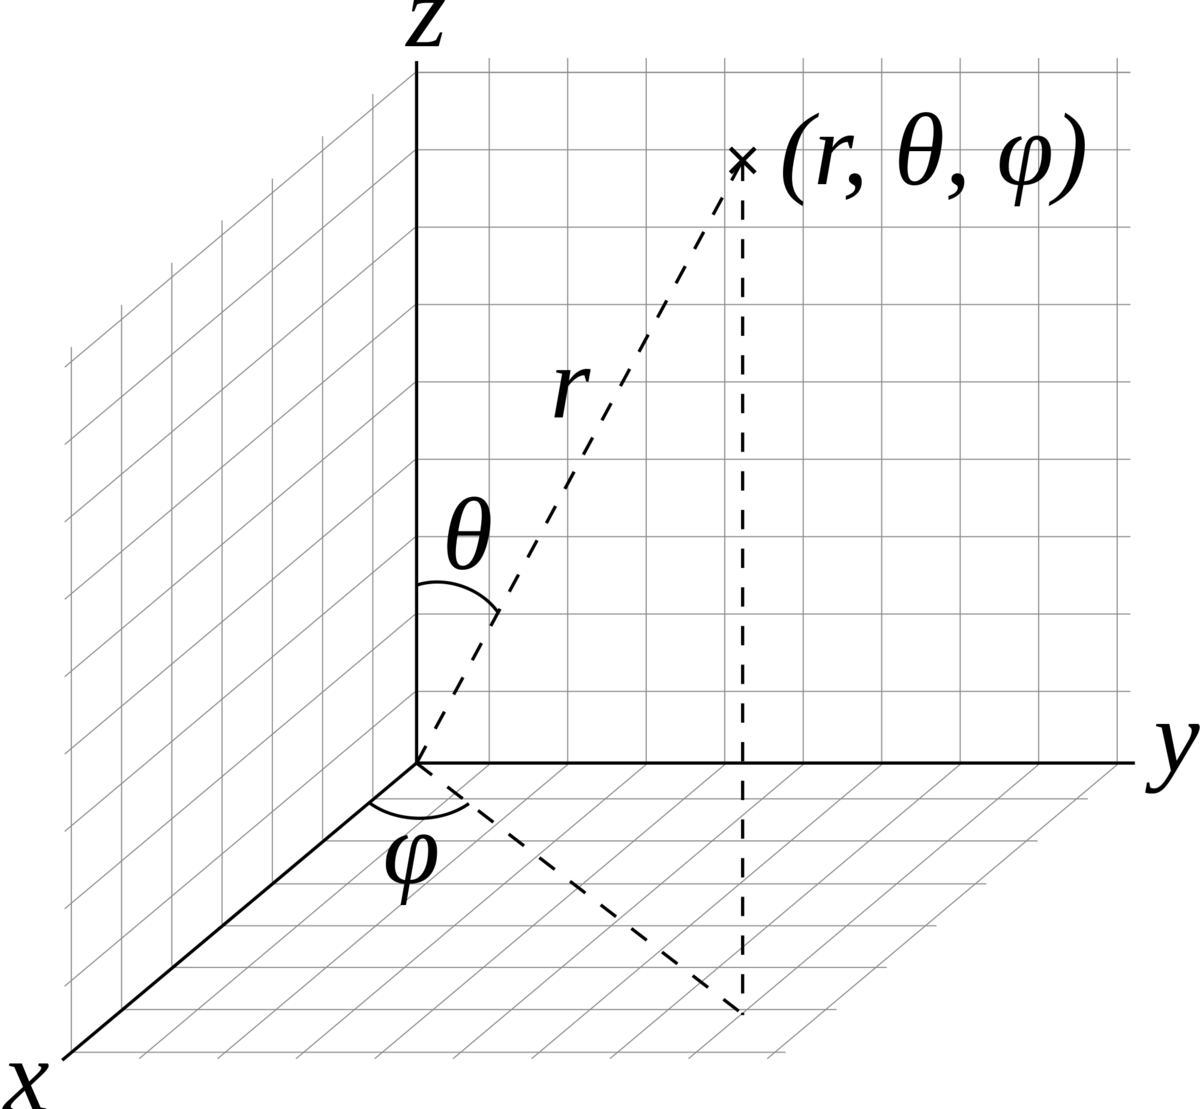
\includegraphics[width=4cm]{images/sphcoord}
\end{center}

\begin{eqnarray}
I 
&=& \frac{1}{3} (I_x + I_y + I_z ) \nn\\
&=& 
\frac{1}{3} \iiint_V \rho(r) (y^2+z^2) dV +
\frac{1}{3} \iiint_V \rho(r) (x^2+z^2) dV +
\frac{1}{3} \iiint_V \rho(r) (x^2+y^2) dV \nn\\
&=&
\frac{1}{3} \iiint_V \rho(r) (2x^2 + 2y^2+2z^2) dV \nn\\
&=&
\frac{2}{3} \iiint_V \rho(r) r^2 dV \nn\\
&=& \frac{2}{3} \iiint_V \rho(r) r^2 r^2 \sin\theta dr \; d\theta \; d\phi \nn\\
&=& \frac{2}{3} \int_0^R \int_0^\pi \int_0^{2\pi}    \rho(r) r^2 r^2 \sin\theta dr \; d\theta \; d\phi \nn\\
&=& \frac{2}{3} \left(\int_0^\pi \sin\theta d\theta \right)
\left( \int_0^{2\pi} d\phi \right)  \int_0^R   \rho(r) r^4 dr \nn\\
&=& \frac{8\pi}{3}  \int_0^R   \rho(r) r^4 dr 
\end{eqnarray}

Alternative solution:
$I$ is evaluated for the special case where the rotation axis is the $z$-axis, 
where $d = r sin\theta$. 
Substitution in $I=\int_V \rho d^2 dV$ yields
\begin{eqnarray}
I
&=& \iiint_V \rho(r) (r^2 \sin^2\theta ) dV  \nn\\
&=& \int_0^R \int_0^\pi \int_0^{2\pi} \rho(r) ( r^2 \sin^2\theta ) r^2 \sin\theta dr \; d\theta \; d\phi \nn\\
&=& \left(\int_0^\pi \sin^3 \theta d\theta \right)
\left( \int_0^{2\pi} d\phi \right)  \int_0^R   \rho(r) r^4 dr \nn
\end{eqnarray}
By writing $\sin^3\theta = \sin\theta (1-\cos^2\theta)$ we can operate a change of variables $u=\cos \theta$,
and we arrive at $\int \sin^3 \theta d\theta=4/3$ (skipping a few steps here) 
and we obtain the expected result.






\newpage
%------------------------------
\subsection{Problem 2}

For a uniform sphere, we have $\rho(r)=\rho_0$. Then 

\begin{eqnarray}
I 
&=& \frac{8\pi}{3}  \int_0^R   \rho_0 r^4 dr \nn\\
&=& \frac{8\pi}{3}\rho_0  \int_0^R  r^4 dr \nn\\
&=& \frac{8\pi}{15}\rho_0 R^5  \int_0^R  r^4 dr \nn
\end{eqnarray}

The mass of the sphere is
\begin{eqnarray}
M 
&=& \iiint_V \rho(r) dV \nn\\
&=& \rho_0 \int_0^R \int_0^\pi \int_0^{2\pi}   r^2 \sin\theta dr \; d\theta \; d\phi \nn\\
&=& \rho_0 \frac{4}{3} \pi R^3
\end{eqnarray}

In the end we get
\[
I = \frac{2}{5} M R^2
\]


When all the mass is concentrated in the center, then $\rho(r)= \rho_0 \delta(r)$ where 
$\delta$ is the Dirac delta function\footnote{\url{https://en.wikipedia.org/wiki/Dirac_delta_function}}.
Then 
\begin{eqnarray}
I 
&=& \frac{8\pi}{3}  \int_0^R   \rho_0 \delta(r) r^4 dr \nn\\
&=& \frac{8\pi}{3} \rho_0  \int_0^R  \delta(r) r^4 dr \nn\\
&=& 0
\end{eqnarray}

When all the mass is concentrated in a shell of zero thickness of radius $R$, 
then $\rho(r)= \rho_0 \delta(r-R)$, so 
\begin{eqnarray}
I 
&=& \frac{8\pi}{3}  \int_0^R   \rho_0 \delta(r-R) r^4 dr \nn\\
&=& \frac{8\pi}{3} \rho_0  \int_0^R  \delta(r-R) r^4 dr \nn\\
&=& \frac{8\pi}{3} \rho_0  R^4
\end{eqnarray}
Conversely, its mass is 
\begin{eqnarray}
M 
&=& \iiint_V \rho(r) dV \nn\\
&=& \rho_0 \int_0^R \int_0^\pi \int_0^{2\pi} \delta(r-R)  r^2 \sin\theta dr \; d\theta \; d\phi \nn\\
&=& \rho_0 4  \pi R^2
\end{eqnarray}
and then 
\[
I = \frac{2}{3} M R^2
\]



\newpage
%------------------------------
\subsection{Problem 3}


\begin{eqnarray}
\langle \rho \rangle 
&=& \frac{1}{V} \iiint_V \rho dV \nn\\
&=& \frac{1}{\frac{4}{3}\pi R^3} \iiint_V \rho(r) r^2 \sin\theta dr \; d\theta d\phi \nn\\
&=& \frac{1}{\frac{4}{3}\pi R^3}  4\pi \int_0^R \rho(r) r^2  dr \nn\\
&=& \frac{3}{R^3}   \int_0^R \rho(r) r^2  dr  \label{appgravsols3}
\end{eqnarray}

We then turn to the moment of inertia:
\begin{eqnarray}
I 
&=& \frac{8\pi}{3} \int_0^R \rho(r) r^4 dr \label{appgravsols2}\\
&=& f M R^2 \label{appgravsols1}
\end{eqnarray}
where 
\[
M 
= \iiint_V \rho(r) dV 
= V \; \underbrace{\frac{1}{V} \iiint_V \rho(r) dV }_{\langle\rho\rangle}
= \frac{4}{3}\pi R^3 \langle\rho\rangle
\]
We then insert this expression of $M$ in Eq.~\eqref{appgravsols1}:
\[
I
= f \frac{4}{3}\pi R^3 \langle\rho\rangle R^2
= f \frac{4}{3}\pi R^5 \langle\rho\rangle 
\]
Equating this to Eq.~\ref{appgravsols2} yields
\[
\frac{8\pi}{3} \int_0^R \rho(r) r^4 dr = f \frac{4}{3}\pi R^5 \langle\rho\rangle
\]
or, 
\begin{equation}
f \langle \rho \rangle R^5 = 2 \int_0^R \rho(r) r^4 dr  \label{appgravsols4}
\end{equation}


We now make use of the expression for the density:
\[
\rho(r) =
\left\{
\begin{array}{ll}
\rho_c & 0\leq r \leq R_c \\
\rho_m & R_c\leq r \leq R 
\end{array}
\right.
\]
Then Eq.~\eqref{appgravsols3} yields
\begin{eqnarray}
\langle \rho \rangle 
&=& \frac{3}{R^3}   \int_0^R \rho(r) r^2  dr \nn\\
&=& \frac{3}{R^3} \left(   \int_0^{R_c} \rho_c r^2  dr +  \int_{R_c}^R \rho_m r^2  dr \right) \nn\\
&=& \frac{3}{R^3} \left(  \frac{R_c^3}{3} \rho_c  +   \frac{1}{3}(R^3-R_c^3) \rho_m \right) \nn\\
&=&   \frac{R_c^3}{R^3} \rho_c  +   (1-\frac{R_c^3}{R^3}) \rho_m  \nn\\
&=&   \left(\frac{R_c}{R}\right)^3 \rho_c  +   \left[1-\left(\frac{R_c}{R}\right)^3\right] \rho_m 
\end{eqnarray}
We know $\rho_m$, but not $\rho_c$, so we write:
\begin{equation}
\rho_c 
=\rho_m \left[ 1 + \left(\frac{R}{R_c}\right)^3 \left(\frac{\langle \rho \rangle}{\rho_m} -1\right) \right]
\label{appgravsols5} 
\end{equation}

We now turn to Eq.~\eqref{appgravsols4}. Since 
\begin{eqnarray}
2 \int_0^R \rho(r) r^4 dr 
&=&   2 \int_0^{R_c} \rho_c r^4 dr +  2 \int_{R_c}^R \rho_m r^4 dr \nn\\
&=& \frac{2}{5} \left[ R_c^5  \rho_c + (R^5-R_c^5) \rho_m  \right]  \nn
\end{eqnarray}
then 
\[
f \langle \rho \rangle R^5 = \frac{2}{5} \left[ R_c^5  \rho_c + (R^5-R_c^5) \rho_m  \right] 
\]
or, 
\[
\frac{5 f \langle \rho \rangle R^5}{2 \rho_m} =   R_c^5  \frac{\rho_c}{\rho_m} + (R^5-R_c^5)  
\]
\[
\frac{5 f \langle \rho \rangle R^5}{2 \rho_m} =   R_c^5  (\frac{\rho_c}{\rho_m}-1) + R^5)  
\]
Now dividing by $R^5$ on each side:
\[
\frac{5 f \langle \rho \rangle }{2 \rho_m} =  \left(\frac{R_c}{R}\right)^5    \left(\frac{\rho_c}{\rho_m}-1 \right) + 1 
\]
Using Eq.~\eqref{appgravsols5}, we can write 
\[
\frac{\rho_c}{\rho_m}-1  = 
\left(\frac{R}{R_c}\right)^3 \left(\frac{\langle \rho \rangle}{\rho_m} -1\right) 
\]
so finally
\[
\frac{5 f \langle \rho \rangle }{2 \rho_m} - 1=  \left(\frac{R_c}{R}\right)^5     
\left(\frac{R}{R_c}\right)^3 \left(\frac{\langle \rho \rangle}{\rho_m} -1\right) 
\]
or, 
\[
\frac{5 f \langle \rho \rangle }{2 \rho_m} - 1=  \left(\frac{R_c}{R}\right)^2     
 \left(\frac{\langle \rho \rangle}{\rho_m} -1\right) 
\]
and then 
\[
\left(\frac{R_c}{R}\right)
=
\left( 
\frac{ \frac{5 f \langle \rho \rangle }{2 \rho_m} - 1  }{  \left(\frac{\langle \rho \rangle}{\rho_m} -1\right)  }
\right)^{1/2}
\]




\newpage
%------------------------------
\subsection{Problem 4}

Assume a uniform mantle $\rho_m$ and core $\rho_c$. For the total mass we have 
\[
M=\int_V \rho dV = 4\pi \int_0^R \rho(r) r^2 dr 
=
\frac{4\pi}{3} R_c^3 \rho_c + \frac{4\pi}{3} (R^3-R_c^3) \rho_m
\]
For the moment of inertia we have,
\[
I 
= \frac{8\pi}{3} \int_0^R \rho(r) r^4 dr
= 
\frac{8\pi}{15} R_c^5 \rho_c + \frac{8\pi}{15} (R^5-R_c^5) \rho_m
\]
In matrix form the above equations become:
\[
\left(
\begin{array}{cc}
\frac{4\pi}{3} R_c^3  & \frac{4\pi}{3} (R^3-R_c^3) \\
\frac{8\pi}{15} R_c^5 &  \frac{8\pi}{15} (R^5-R_c^5) 
\end{array}
\right)
\cdot
\left(
\begin{array}{cc}
\rho_c \\ \rho_m
\end{array}
\right)
=
\left(
\begin{array}{cc}
M & I
\end{array}
\right)
\]
We use Cramers rule
\[
\left(
\begin{array}{cc}
a11 & a12 \\
a21 & a22
\end{array}
\right)
\cdot
\left(
\begin{array}{c}
x_1 \\ x_2
\end{array}
\right)
=
\left(
\begin{array}{c}
b_1 \\ b_2
\end{array}
\right)
\qquad
\Rightarrow
\qquad
\left(
\begin{array}{c}
x_1 \\ x_2
\end{array}
\right)
=
\frac{1}{\Delta}
\left(
\begin{array}{cc}
a22 & -a12 \\
-a21 & a11
\end{array}
\right)
\cdot
\left(
\begin{array}{c}
b_1 \\ b_2
\end{array}
\right)
\]
In our case the determinant of the matrix is 
\[
\Delta = \frac{32\pi^2}{45}\left[ R_c^3(R^5-R_c^3)-R_c^5(R^3-R_c^3)   \right]
\]



%------------------------------
\subsection{Problem 5}

skipped 

%------------------------------
\subsection{Problem 6}

see lecture notes


%------------------------------
\subsection{Problem 7}

\[
g = \frac{{\cal G}M}{R^2} = \frac{6.67e-11*5.97e24}{6371000^2} \simeq 9.8
\]

%------------------------------
\subsection{Problem 8}

\[
p_{CMB} = \int \rho g dz \simeq \rho_0 g_0 (R_{Earth}-R_{CMB}) \simeq 127.5GPa
\]


\newpage
%------------------------------
\subsection{Problem 9}

\[
U(\vec{r}) 
= -\frac{{\cal G} m_1}{|\vec{r}_1 - \vec{r}|} 
= -\frac{{\cal G} m_1}{\sqrt{(x_1-x)^2+(y_1-y)^2+(z_1-z)^2}} 
\]

\[
\vec\nabla U = 
\left(
\begin{array}{c}
\partial_x U \\
\partial_y U \\
\partial_z U 
\end{array}
\right)
\]

We have 
\begin{eqnarray}
\partial_x U 
&=&  -{\cal G} m_1 \frac{\partial }{\partial x} \frac{1}{\sqrt{(x_1-x)^2+(y_1-y)^2+(z_1-z)^2}} \nn\\
&=&  -{\cal G} m_1 \cdot -\frac{1}{2}  \frac{-2(x_1-x)}{[(x_1-x)^2+(y_1-y)^2+(z_1-z)^2]^{3/2}} \nn\\
&=&  {\cal G} m_1  \frac{1}{[(x_1-x)^2+(y_1-y)^2+(z_1-z)^2]} \frac{-(x_1-x)}{\sqrt{(x_1-x)^2+(y_1-y)^2+(z_1-z)^2}} \nn\\
&=&  {\cal G} m_1  \frac{1}{|\vec{r}_1 - \vec{r}|^2} \frac{-(x_1-x)}{\sqrt{(x_1-x)^2+(y_1-y)^2+(z_1-z)^2}} \nn
\end{eqnarray}
We repeat this operation for $\partial_y$ and $\partial_z$ and finally:

\[
-\vec\nabla U = 
\left(
\begin{array}{c}
\partial_x U \\
\partial_y U \\
\partial_z U 
\end{array}
\right)
=  {\cal G} m_1  \frac{1}{|\vec{r}_1 - \vec{r}|^2} 
\left(
\begin{array}{c}
\frac{(x_1-x)}{|\vec{r}_1 - \vec{r}|} \\
\frac{(y_1-y)}{|\vec{r}_1 - \vec{r}|} \\
\frac{(z_1-z)}{|\vec{r}_1 - \vec{r}|} \\
\end{array}
\right)
=
\frac{ {\cal G} m_1}{|\vec{r}_1 - \vec{r}|^2} \vec{e}_{\vec{r}_1\vec{r}} = \vec{g}
\]


%------------------------------
\subsection{Problem 10}

\[
\int_V \Delta U dV
=
\int_V 4\pi {\cal G} \rho dV
=
4\pi {\cal G} \int_V M \delta(\vec{r}-\vec{r}_0) dV
=
4 \pi {\cal G} M
\] 


\[
\int_V \Delta U dV 
=
\int_V \vec\nabla^2 U dV
=
\int_V \vec\nabla \cdot \vec\nabla U dV
=
\int_\Gamma \vec\nabla U \cdot \vec n dS
=
\int_\Gamma ( - \vec{g}) \cdot \vec n dS
=
\int_\Gamma g  dS
=
4\pi r^2 g
\]

Note that we have $\vec{g}$ which is pointing towards the center and therefore has the 
opposite direction to $\vec{n}$ which is normal to the shell surface so that $( - \vec{g}) \cdot \vec n = g$.
Also the integral on $\Gamma$ is at constant radius so $g(r)$ can be taken out of the integral.

Finally we obtain 
\[
g = \frac{{\cal G} M}{r^2}
\]

%------------------------------
\subsection{Problem 11}

We start from  $ \vec\nabla^2 U = 4\pi {\cal G}\rho $.
We then have 
\[
[\vec\nabla^2] [U] = [{\cal G}][\rho ]
\]
so 
\[
[U]=  [{\cal G}][\rho ] / [\vec\nabla^2]
= M^{-1} L^3 T^{-2} \cdot M L^{-3} \cdot L^2
= L^2 T^{-2} 
= \underbrace{ML^2 T^{-2}}_{energy} / M 
\]
(see lecture notes on physical dimensions)

%------------------------------
\subsection{Problem 12}

Escape velocity is speed at which kinetic energy is equal to gravitational 
potential energy, i.e. 
\[
\frac{1}{2}m v^2 = m g H
\]
so $v=\sqrt{2gH}$ and since $g={\cal G}M/R^2$
then the escape velocity at the surface (i.e. $H=R$) is given by
\[
v = \sqrt{2 {\cal G} M/ R}
\]

\[
v_{earth} \simeq 11.2 km/s
\]
\[
v_{moon} \simeq 2.4 km/s
\]

See \url{https://www.newworldencyclopedia.org/entry/Escape_velocity}

%------------------------------
\subsection{Problem 13}

\begin{eqnarray}
E 
&=& - \int_V \rho U dV \nn\\
&=& - \int_V \rho_0  U(r) r^2 \sin\theta \; dr d\theta d\phi \nn\\
&=& - 4 \pi \rho_0 \int_0^R r^2 U(r) dr \nn\\
&=& - 4\pi\rho_0 \int_0^R r^2 \left[ \frac{2\pi}{3}{\cal G} \rho_0 r^2 - \frac{3}{2} \frac{{\cal G} M}{R}  \right] dr \nn\\
&=& - \frac{8\pi^2\rho_0^2}{3} {\cal G} \int_0^R r^4 dr  
+ 6 \rho_0 \pi  \frac{{\cal G} M}{R} \int_0^R r^2  dr \nn\\
&=& ... \nn\\
&=& \frac{8 \pi}{5} \rho_0 M R^2 {\cal G}
\end{eqnarray}

%------------------------------
\subsection{Problem 14}

We start from the Laplace operator in spherical coordinates:
\[
\Delta = \frac{1}{r^2} \frac{\partial }{\partial r}\left( r^2 \frac{\partial }{\partial r}\right)
+\frac{1}{r^2 \sin\theta} \frac{\partial }{\partial \theta}
\left(
\sin\theta \frac{\partial }{\partial\theta}
\right)
+ \frac{1}{r^2 \sin^2\theta} \frac{\partial^2 }{\partial\phi^2}
\]
Because of the symmetry of the problem, the solution is expected to only depend on $r$, and not on $\theta$
nor $\phi$, so that $\partial_\theta \rightarrow 0$ and $\partial_\phi \rightarrow 0$ in the equation above. 
We end up with:
\[
\Delta = \frac{1}{r^2} \frac{\partial }{\partial r}\left( r^2 \frac{\partial }{\partial r}\right)
\]
Inside the planet, the density is not zero, so we need to solve a Poisson equation
\[
\Delta U = \frac{1}{r^2} \frac{\partial }{\partial r}\left( r^2 \frac{\partial U}{\partial r}\right)
= 4 \pi {\cal G} \rho_0  
\]
Outside the planet the density is zero and we need to solve a Laplace equation:
\[
\Delta U = \frac{1}{r^2} \frac{\partial }{\partial r}\left( r^2 \frac{\partial U}{\partial r}\right)
= 0 
\]

We start with the Poisson equation which we rewrite as follows:
\[
\frac{\partial }{\partial r}\left( r^2 \frac{\partial U}{\partial r}\right)
= 4 \pi {\cal G} \rho_0 r^2 
\]
We integrate once and obtain
\[
r^2 \frac{\partial U}{\partial r}
= \frac{4 \pi}{3} {\cal G} \rho_0 r^3 + A 
\]
where $A$ is a constant to be specified later. We divide by $r^2$ and obtain 
\[
\frac{\partial U}{\partial r}
= \frac{4 \pi}{3} {\cal G} \rho_0 r + \frac{A}{r^2}
\]
The radial component of the gradient operator is simply $\partial_r$ so that the equation 
above is (save a minus sign) $g_r$:
\[
g_r(r) = - \frac{4 \pi}{3} {\cal G} \rho_0 r - \frac{A}{r^2}
\]
When $r\rightarrow 0$ the gravity acceleration must remain finite so we need to set $A=0$. Then 
\[
\boxed{
g_r(r)|_{inside} = - \frac{4 \pi}{3} {\cal G} \rho_0 r 
}
\]
We integrate once more and obtain 
\[
U(r)|_{inside} = \frac{2\pi}{3}{\cal G} \rho_0 r^2 + B
\]
where $B$ is a constant.

We now turn to the Laplace equation outside the planet which yields
\[
r^2 \frac{\partial U}{\partial r}  = C 
\]
where $C$ is a constant. Then it follows that 
\[
\frac{\partial U}{\partial r}  = \frac{C}{r^2} 
\]
or, 
\[
U(r) = -\frac{C}{r} + D
\]
When $r \rightarrow \infty$ the potential tends to zero, so that $D=0$. 
Then 
\[
\boxed{
U(r)_{outside} = -\frac{C}{r}
}
\]
and from $g_r(r)=-\partial_r U$ we get
\[
g_r(r)|_{outside} = -\frac{C}{r^2}
\]

We have solved the Poisson and Laplace equations but remain two constants to be specified. 
In order to do so we invoke the continuity of the gravity acceleration and potential at the 
surface of the planet:
\begin{eqnarray}
g_r(r=R)|_{inside}&=&g_r(r=R)|_{outside} \nn\\
U(r=R)|_{inside}&=&U(r=R)|_{outside} \nn
\end{eqnarray}

The first continuity condition yields
\[
-\frac{C}{R^2} = -\frac{4\pi}{3} {\cal G} \rho_0 R
\]
i.e., $C = M {\cal G}$. 
The second continuity condition then yields
\[
-\frac{C}{R} = -\frac{M {\cal G}}{R} = 
\frac{2\pi}{3}{\cal G} \rho_0 R^2 + B
\]
i.e. $B = -\frac32 \frac{M {\cal G}}{R}$.

If all the mass is concentrated at the origin then by definition
\[
g_r(r) = \frac{M {\cal G}}{r^2} 
\qquad
U(r) = -\frac{M {\cal G}}{R} 
\]

Finally
\[
P(r) = -\int_r^R \rho(r') g(r') dr' = \int_r^R \rho_0 \frac{4\pi}{3} {\cal G} \rho_0 r' dr' 
= \frac{2 \pi}{3} {\cal G} \rho_0^2 (R^2-r^2)
\]

\begin{comment}

%------------------------------
\subsection{Problem 15}

We start from \eqref{equiv_potential}, i.e
\[
U(r)   = - \int_r^{\infty} \frac{Gm(r')}{r'^2} dr'
\]

Outside the sphere, $r>R$ and the mass at any location $r'>R$ is simply $M$.
Then 
\[
U(r)   = - \int_r^{\infty} \frac{GM}{r'^2} dr' = -\frac{{\cal G}M}{r}
\]


When $r<R$ we can split the integral in two:
\[
U(r)   = - \int_r^{R} \frac{Gm(r')}{r'^2} dr'  - \int_R^{\infty} \frac{Gm(r')}{r'^2} dr'
\]
We have just computed the second term so we focus on the first one. In this integral the mass 
$m(r')= \frac{4}{3}\pi r'^3 \rho_0$ so that 
\[
U(r)   = - \int_r^{R} \frac{G}{r'^2} \frac{4}{3}\pi r'^3 \rho_0  dr'   -\frac{{\cal G}M}{r} 
=-\frac{1}{2} \frac{4}{3}\pi {\cal G} (R^2-r^2)  -\frac{{\cal G}M}{r}
= \frac{2\pi}{3} \rho_0 {\cal G} r^2 - \frac{3}{2} \frac{{\cal G}M}{r}
\]


\end{comment}
